\begin{blocksection}
\question Define the function \texttt{factor\_tree} which takes in a positive integer \texttt{n} and returns a factor tree for \texttt{n}. In a factor tree, multiplying the leaves together is the prime factorization of the root, \texttt{n}. See below for an example of a factor tree for \texttt{n = 20}.
\begin{center}
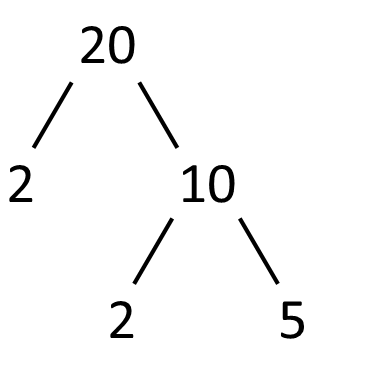
\includegraphics[scale=0.3]{factor_tree_20.png}
\end{center}

\vspace{2\baselineskip}
\begin{lstlisting}
def factor_tree(n):
     """
     >>> factor_tree(20)
     Tree(20, [Tree(2), Tree(10, [Tree(2), Tree(5)])])
     >>> factor_tree(1)
     Tree(1)

    for i in ______________________:

        if ________________________:

            return Tree(_____, _____________________________)

    _______________________________
\end{lstlisting}

\begin{solution}[0.5in]
\begin{lstlisting}
    for i in range(2, n):
        if n % i == 0:
            return Tree(n, [Tree(i), factor_tree(n // i)])
    return Tree(n)
\end{lstlisting}
\end{solution}
\begin{guide}
\textbf{Teaching Tips}
    \begin{itemize}
        \item Remind students that for loops can used on ranges since they will want to look for a list to iterate through.
        \item Students are often disoriented to see recursive problems without evident base cases. Make sure to emphasize how the if condition protects the function from infinite recursion.
        \item The order of this function can be a bit confusing, with the simplest case (if there are no factors) being put at the end. It might be good to walk through the thought process before getting into the code.
    \end{itemize}
\end{guide}
\end{blocksection}
